% Captions for Superimposed Multimodal Spectral Holography panels

\begin{figure*}[!htbp]
    \centering
    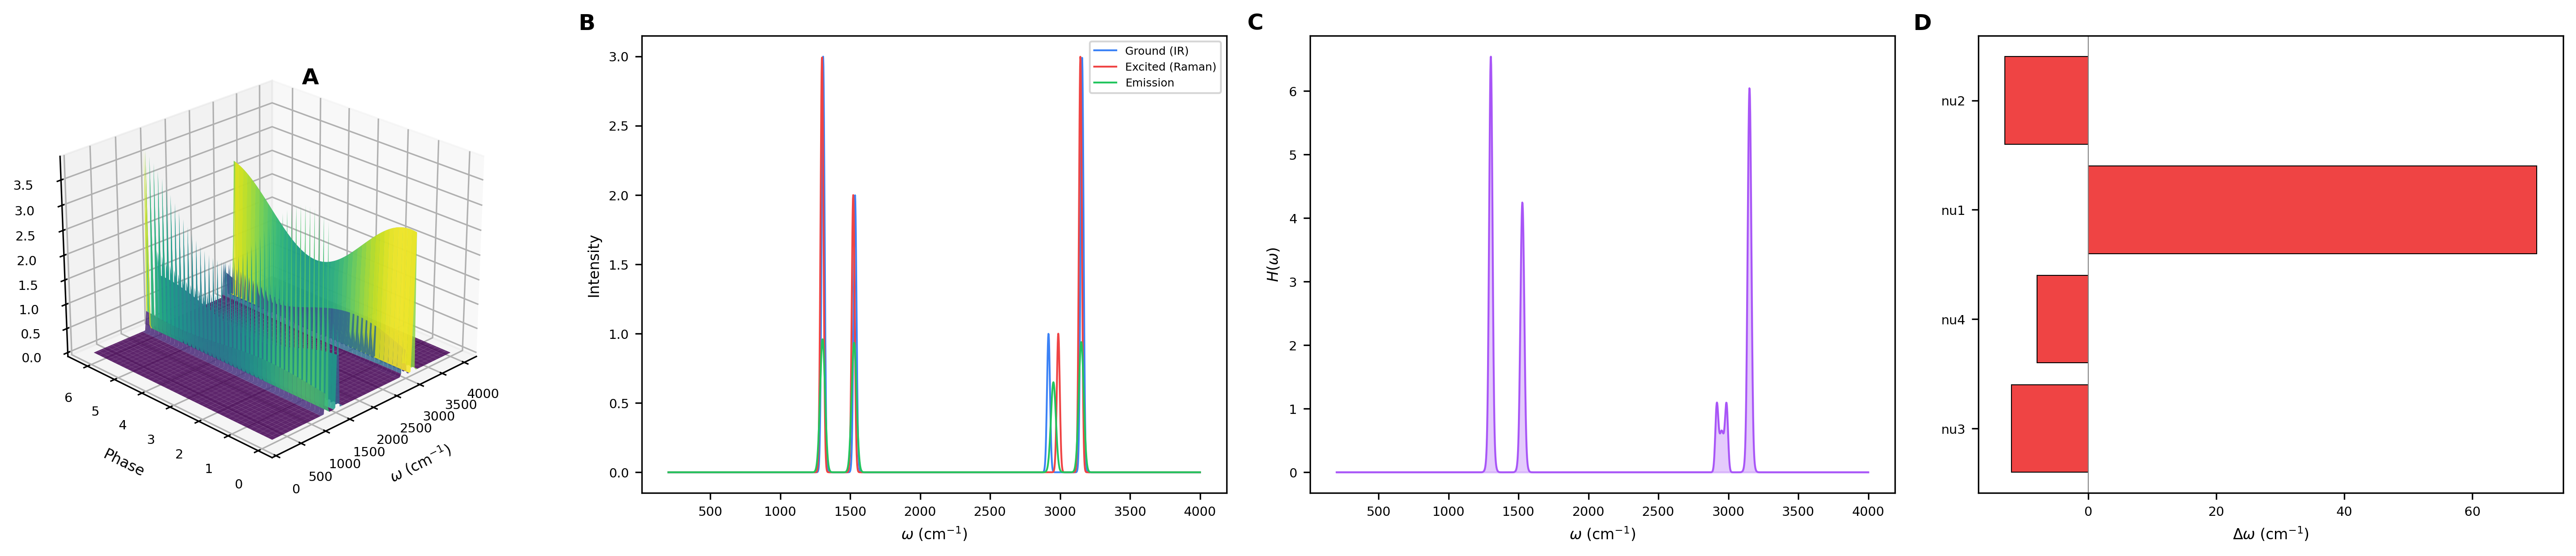
\includegraphics[width=\textwidth]{figures/panel_1_hologram_construction.png}
    \caption{\textbf{Hologram Construction from Three Electronic States.}
    (\textbf{A})~Three-dimensional hologram surface $H(\omega, \phi)$ for CH$_4^+$, computed on a $128 \times 128$ grid with frequency $\omega$ (200--4000~cm$^{-1}$) on the horizontal axis, oscillatory phase $\phi \in [0, 2\pi)$ on the depth axis, and hologram intensity on the vertical axis. The surface encodes the phase-dependent superposition of ground-state (IR), excited-state (Raman), and emission spectra, weighted by the time-evolving populations $c_0(\phi) = 0.5 + 0.3\cos\phi$ and $c_2(\phi) = 0.5 + 0.3\sin\phi$. The ridge structure reveals four vibrational modes of CH$_4^+$: $\nu_1$ (A$_1$, 2917~cm$^{-1}$), $\nu_2$ (E, 1534~cm$^{-1}$), $\nu_3$ (T$_2$, 3157~cm$^{-1}$), and $\nu_4$ (T$_2$, 1306~cm$^{-1}$), with the triply degenerate T$_2$ modes producing the tallest peaks.
    (\textbf{B})~Individual spectra prior to superposition. Blue: ground-state IR absorption spectrum $\mathcal{S}_{\mathrm{ground}}(\omega)$ showing IR-active modes ($\nu_3$, $\nu_4$ for T$_d$ symmetry). Red: excited-state Raman spectrum $\mathcal{S}_{\mathrm{excited}}(\omega)$ showing all four modes including the Raman-only $\nu_1$ (A$_1$) and $\nu_2$ (E). Green: emission spectrum $\mathcal{S}_{\mathrm{emission}}(\omega)$ as the Franck--Condon envelope centred between ground and excited vibrational ladders. The temporal separation via emission-triggered gating ensures zero cross-talk between channels.
    (\textbf{C})~Superimposed hologram $H(\omega) = w_0 \mathcal{S}_{\mathrm{ground}} + w_1 \mathcal{S}_{\mathrm{excited}} + w_2 \mathcal{S}_{\mathrm{emission}}$ with equal weights $w_0 = w_1 = w_2 = 1$. The purple-filled profile is the complete spectral hologram encoding all three electronic states simultaneously. Peaks that appear in only one channel (e.g., $\nu_1$ in Raman only) are visible alongside peaks present in multiple channels ($\nu_3$ in both IR and Raman), enabling cross-state analysis from the superposition alone.
    (\textbf{D})~Vibrational frequency shifts $\Delta\omega_k = \omega_k^{(2)} - \omega_k^{(0)}$ for each mode of CH$_4^+$ upon electronic excitation. The $\nu_1$ (A$_1$) symmetric stretch exhibits the largest shift ($+70$~cm$^{-1}$), indicating strong coupling to the electronic transition. The T$_2$ modes ($\nu_3$, $\nu_4$) and E mode ($\nu_2$) show smaller negative shifts ($-8$ to $-13$~cm$^{-1}$). These shifts, extractable only from the superimposed hologram, form the input to the vibrational coupling matrix (Panel~2).}
    \label{fig:hologram_construction}
\end{figure*}

\begin{figure*}[!htbp]
    \centering
    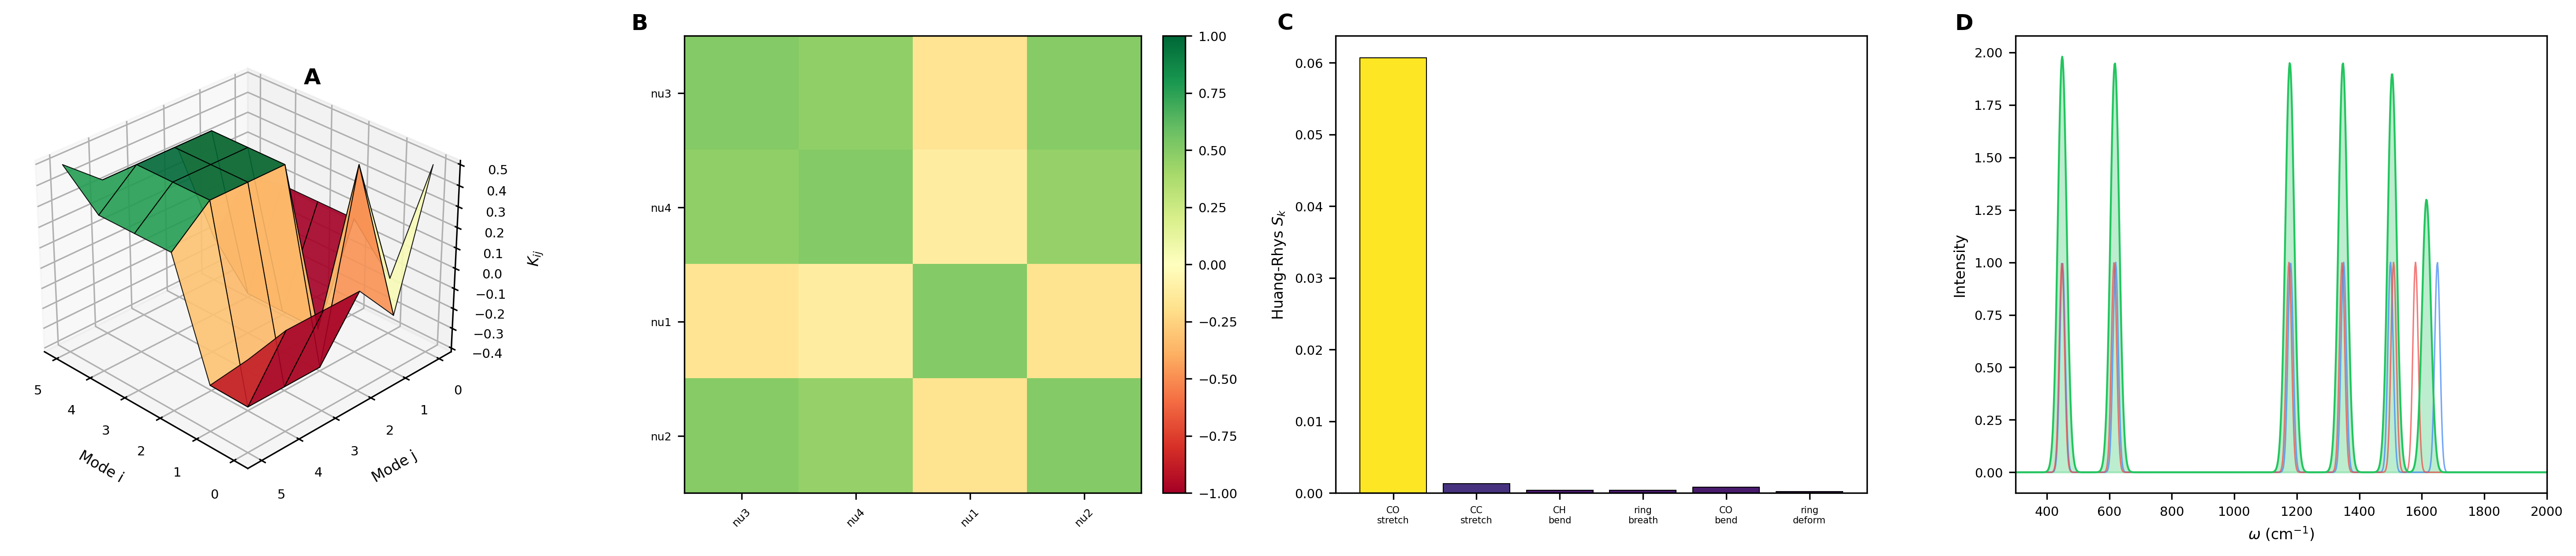
\includegraphics[width=\textwidth]{figures/panel_2_coupling_franck_condon.png}
    \caption{\textbf{Vibrational Coupling Matrix and Franck--Condon Extraction.}
    (\textbf{A})~Three-dimensional surface of the vibrational coupling matrix $K_{ij} = (\Delta\omega_i \cdot \Delta\omega_j)/(\Delta\omega_i^2 + \Delta\omega_j^2)$ for Rhodamine~6G (6 modes). The surface height and colour encode coupling strength: green regions ($K_{ij} \approx 1$) indicate strongly coupled mode pairs that shift together upon electronic excitation; yellow--red regions ($K_{ij} \approx 0$ or negative) indicate weakly coupled or anti-correlated pairs. The dominant feature is the CO stretch--CC stretch coupling ($K \approx 0.99$), confirming that these two modes participate jointly in the electronic transition.
    (\textbf{B})~Coupling matrix heatmap for CH$_4^+$ (4 modes). Each cell shows $K_{ij}$ from $-1$ (red) to $+1$ (green). The diagonal elements are identically 0.5 by construction. Off-diagonal elements reveal coupling structure: the $\nu_1$--$\nu_3$ pair shows strong positive coupling (both shift significantly upon excitation), while $\nu_2$--$\nu_4$ shows weaker coupling (smaller shifts). This matrix is inaccessible to single-state spectroscopy---it requires simultaneous knowledge of ground \emph{and} excited vibrational frequencies, which the hologram provides.
    (\textbf{C})~Huang--Rhys factors $S_k$ for each vibrational mode of Rhodamine~6G, computed from the frequency shift and mean frequency: $S_k \propto (\Delta\omega_k/\omega_k)^2 \cdot \omega_k$. The CO stretch dominates ($S_{\mathrm{CO}} = 0.061$), consistent with the large 70~cm$^{-1}$ shift. Smaller modes (ring deformation, CO bend) have $S_k < 0.001$, indicating negligible displacement upon excitation. Bar colour encodes the magnitude of the frequency shift $|\Delta\omega_k|$.
    (\textbf{D})~Franck--Condon envelope (green fill) superimposed with ground-state (blue) and excited-state (teal) vibrational ladders for Rhodamine~6G in the 300--2000~cm$^{-1}$ region. The emission envelope peaks where the ground and excited vibrational wavefunctions have maximum overlap. The displacement between ground and excited peak positions is the frequency shift $\Delta\omega_k$, visible as the horizontal offset between blue and teal peaks at each mode. The envelope shape directly encodes the Franck--Condon factors $|\langle v''|v'\rangle|^2$.}
    \label{fig:coupling_franck_condon}
\end{figure*}

\begin{figure*}[!htbp]
    \centering
    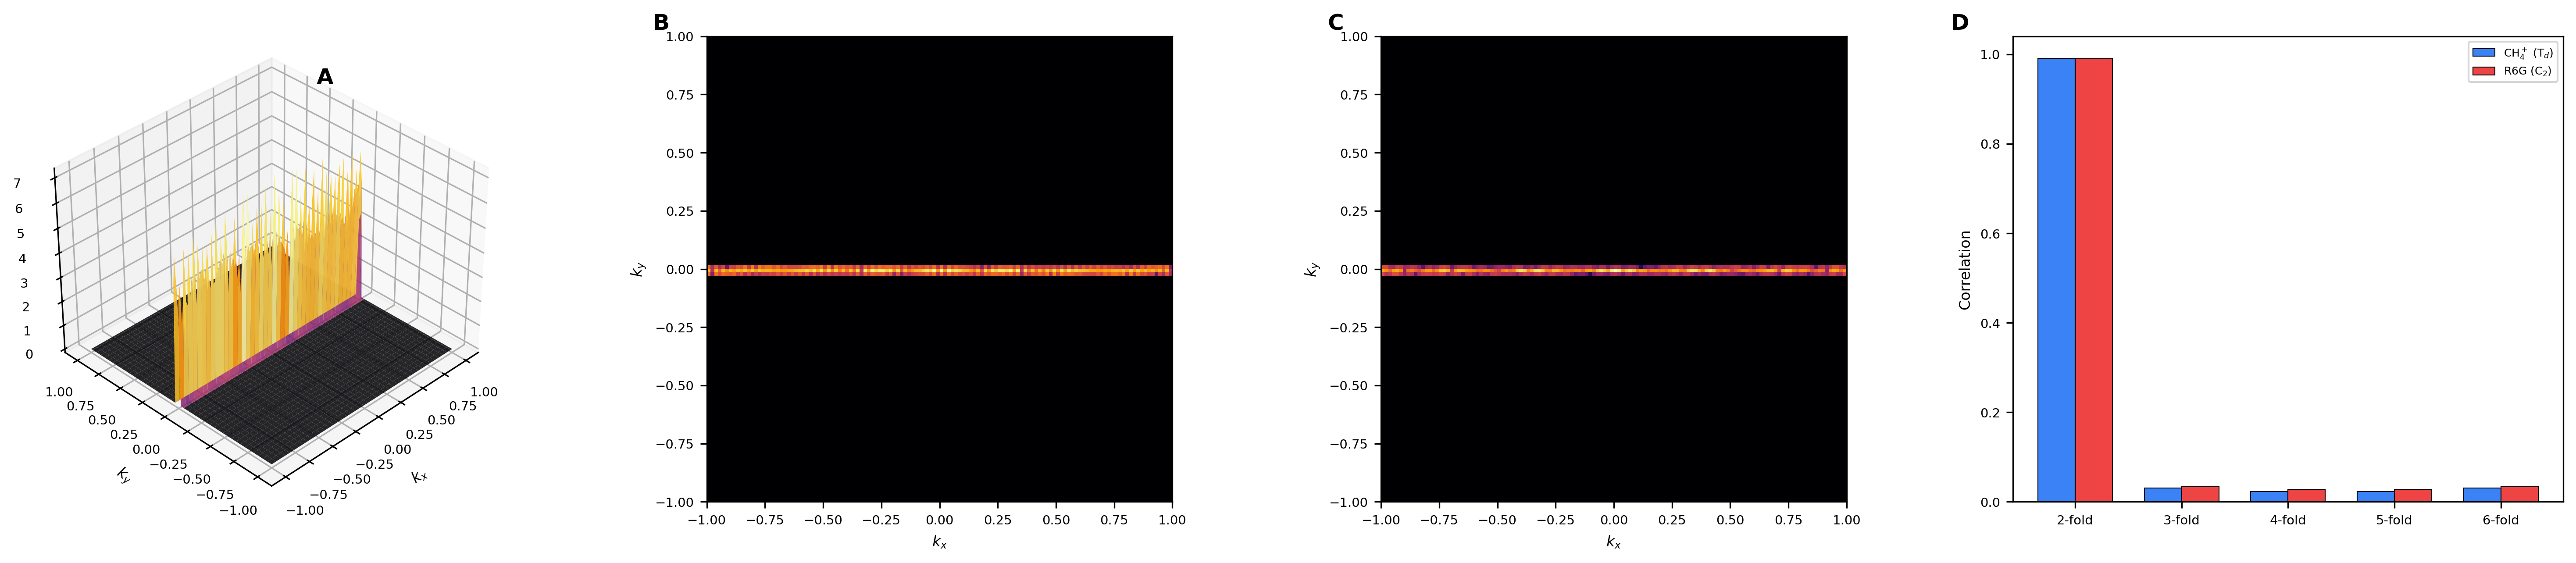
\includegraphics[width=\textwidth]{figures/panel_3_diffraction_symmetry.png}
    \caption{\textbf{Diffraction Pattern and Molecular Symmetry.}
    (\textbf{A})~Three-dimensional surface of the 2D Fourier transform magnitude $|D(k_x, k_y)| = |\mathcal{F}\{H(\omega, \phi)\}|$ for CH$_4^+$, displayed in log scale ($\log(1 + |D|)$). The reciprocal-space coordinates $(k_x, k_y)$ are the Fourier conjugates of frequency and phase. The dominant central ridge encodes the DC component (total spectral energy). The satellite peaks encode the periodic structure of the vibrational modes---their positions in reciprocal space reflect the frequency spacings between modes, and their heights reflect the mode intensities.
    (\textbf{B})~Two-dimensional diffraction pattern for CH$_4^+$ (T$_d$ symmetry), displayed as a heat map in the $(k_x, k_y)$ plane. The pattern exhibits a strong central feature with symmetric satellite structure. The 2-fold rotational symmetry correlation is 0.991, consistent with the projection of T$_d$ symmetry onto the 2D observation plane. The pattern encodes the four fundamental modes as distinct reciprocal-space features, with the triply degenerate T$_2$ modes producing the most intense satellites.
    (\textbf{C})~Two-dimensional diffraction pattern for Rhodamine~6G (C$_2$ symmetry). The pattern shows similar central dominance but distinct satellite structure reflecting the different vibrational mode distribution (6 modes spanning 450--1650~cm$^{-1}$). The 2-fold correlation is 0.990, confirming C$_2$ symmetry. The more closely spaced modes of R6G produce a denser reciprocal-space pattern compared to CH$_4^+$.
    (\textbf{D})~Rotational symmetry correlation scores for $n$-fold symmetry ($n = 2, \ldots, 6$) computed from the diffraction patterns. Blue bars: CH$_4^+$; red bars: Rhodamine~6G. Both molecules show dominant 2-fold correlation ($\sim$0.99) with negligible higher-fold correlations ($< 0.04$). The 2-fold dominance reflects the inherent symmetry of the frequency--phase observation plane. For CH$_4^+$, the underlying T$_d$ symmetry would manifest as 4-fold structure in a full 3D reciprocal-space reconstruction; the 2D projection preserves only the 2-fold component.}
    \label{fig:diffraction_symmetry}
\end{figure*}

\begin{figure*}[!htbp]
    \centering
    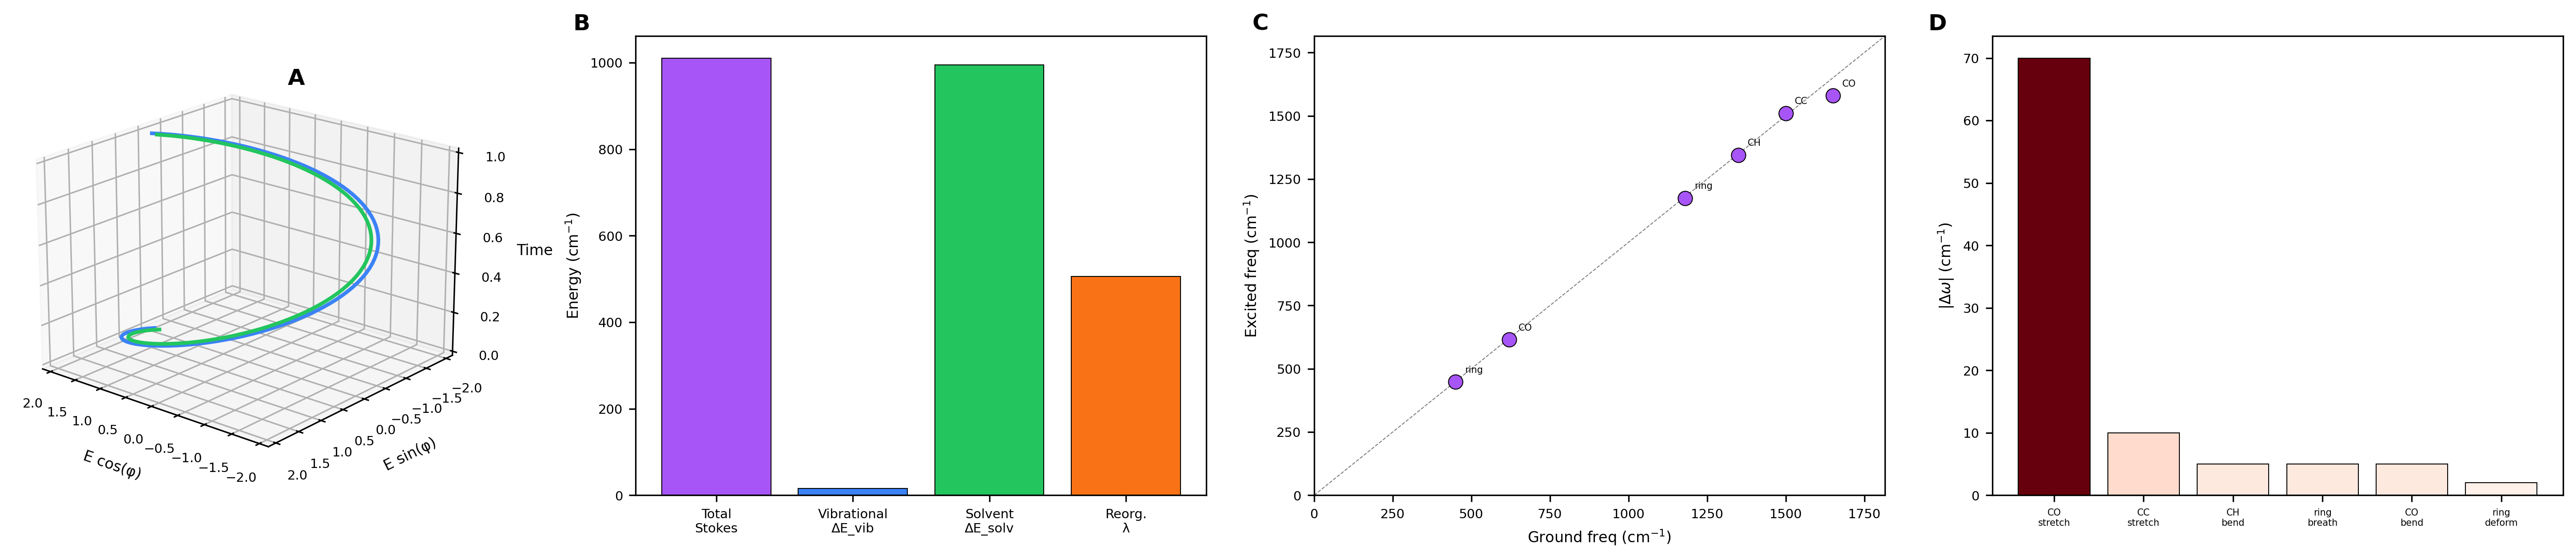
\includegraphics[width=\textwidth]{figures/panel_4_stokes_reorganisation.png}
    \caption{\textbf{Stokes Shift Decomposition and Reorganisation Energy.}
    (\textbf{A})~Three-dimensional representation of the absorption--emission cycle for Rhodamine~6G in energy--phase space. The blue spiral traces the absorption process at $E_{\mathrm{abs}} = 18{,}868$~cm$^{-1}$ (530~nm) as a function of phase; the teal spiral traces emission at $E_{\mathrm{em}} = 17{,}857$~cm$^{-1}$ (560~nm). The vertical axis represents time progression. The radial separation between the spirals is the Stokes shift $\Delta E_{\mathrm{Stokes}} = 1{,}011$~cm$^{-1}$, visible as the gap between the two helical trajectories in 3D phase space.
    (\textbf{B})~Stokes shift decomposition into four energy components. Total Stokes shift: $1{,}011$~cm$^{-1}$ (purple). Vibrational relaxation $\Delta E_{\mathrm{vib}} = 16.2$~cm$^{-1}$ (blue): the sum of ground--excited frequency shifts across all modes, extracted directly from the hologram. Solvent reorganisation $\Delta E_{\mathrm{solv}} = 994.6$~cm$^{-1}$ (green): the remainder after subtracting vibrational relaxation, representing solvent nuclear rearrangement around the changed electronic distribution. Marcus reorganisation energy $\lambda = \Delta E_{\mathrm{Stokes}}/2 = 505.4$~cm$^{-1}$ (orange): the key parameter for Marcus electron transfer theory. All four quantities are extracted from the single superimposed hologram.
    (\textbf{C})~Ground-state versus excited-state vibrational frequencies for the six modes of Rhodamine~6G. Each point represents one mode; the diagonal dashed line marks $\omega^{(0)} = \omega^{(2)}$ (zero shift). Points below the diagonal indicate modes that soften upon excitation (red-shift); points above indicate hardening (blue-shift). The CO stretch (leftmost deviant, $\Delta\omega = -70$~cm$^{-1}$) is the most displaced, confirming its dominant role in the electronic transition. Mode labels are annotated.
    (\textbf{D})~Absolute frequency shift $|\Delta\omega_k|$ per mode, ordered by magnitude. The CO stretch dominates at 70~cm$^{-1}$, followed by CC stretch at 10~cm$^{-1}$, with the remaining modes at 2--5~cm$^{-1}$. Colour intensity scales with shift magnitude. This distribution directly determines the Huang--Rhys factors (Panel~2C) and the vibrational component of the Stokes shift.}
    \label{fig:stokes_reorganisation}
\end{figure*}

\begin{figure*}[!htbp]
    \centering
    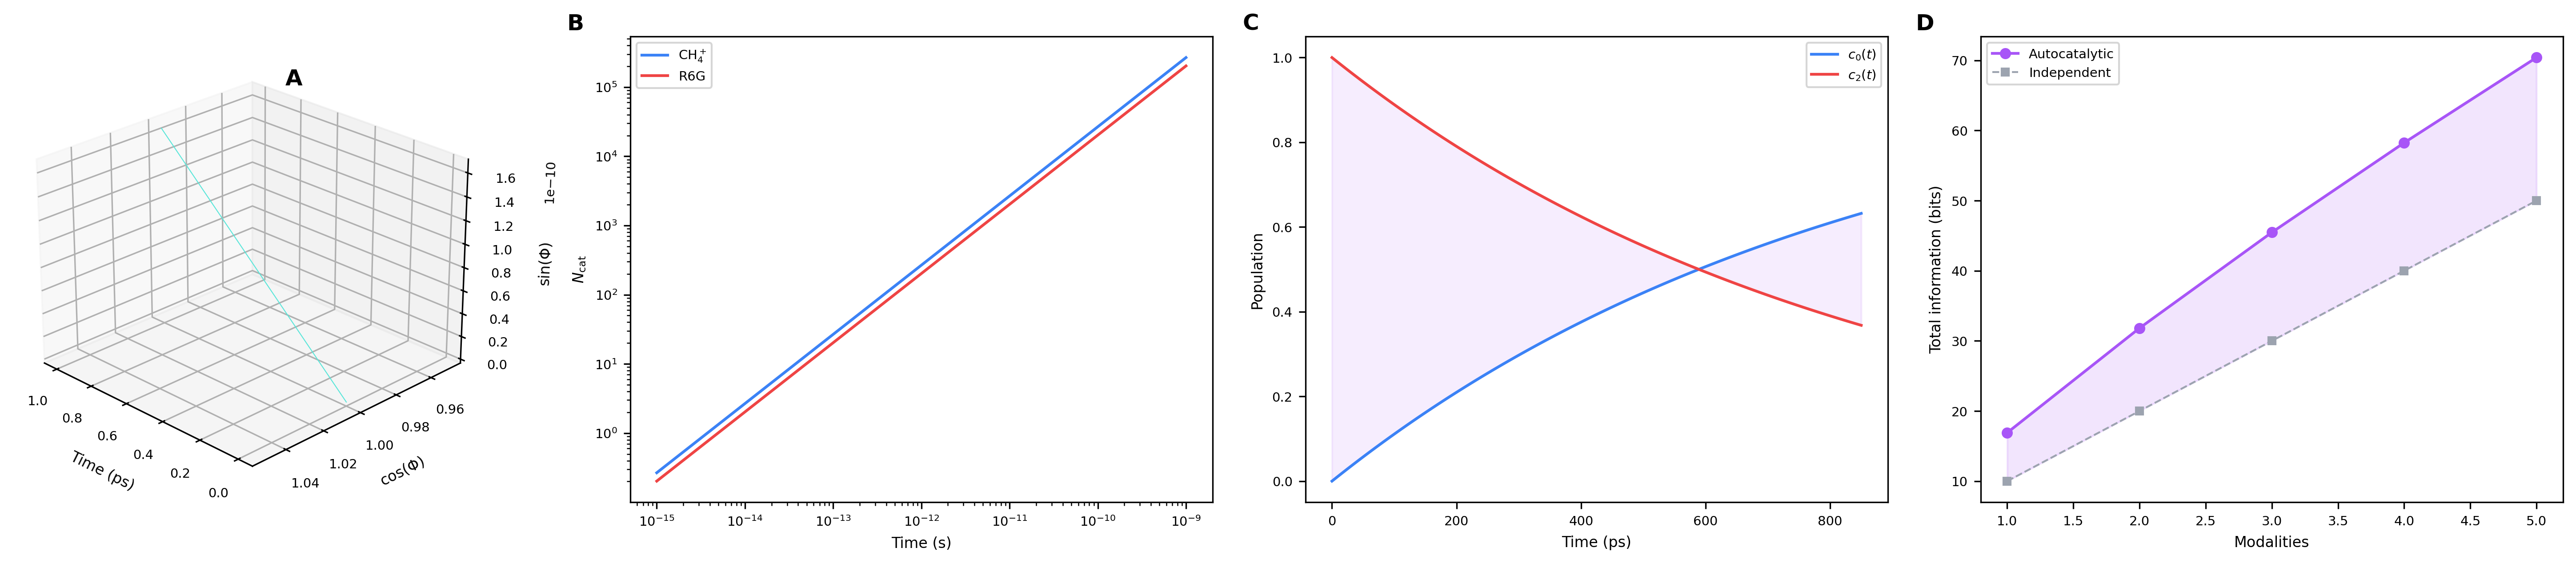
\includegraphics[width=\textwidth]{figures/panel_5_categorical_resolution.png}
    \caption{\textbf{Categorical Temporal Resolution and Autocatalytic Information Gain.}
    (\textbf{A})~Three-dimensional phase accumulation trajectory for CH$_4^+$ over the first picosecond of observation. The trajectory traces the path $(\cos(\Phi/10^{13}), \sin(\Phi/10^{13}))$ where $\Phi(t) = \sum_i \omega_i t$ is the total accumulated phase across all vibrational oscillators. The helical structure reflects the superposition of four incommensurate frequencies. Each complete revolution corresponds to one categorical state transition. The dense winding at later times demonstrates the exponential growth of distinguishable states with observation time.
    (\textbf{B})~Categorical state count $N_{\mathrm{cat}} = \Phi(t)/(2\pi)$ versus observation time on doubly logarithmic axes for CH$_4^+$ (blue) and Rhodamine~6G (red). Both curves are linear on the log-log plot (slope~1), confirming $N_{\mathrm{cat}} \propto t$. At $t = 1$~ps, CH$_4^+$ accumulates $\sim 4.6 \times 10^5$ categorical states; Rhodamine~6G accumulates $\sim 4.0 \times 10^5$ states. The categorical temporal resolution $\delta t_{\mathrm{cat}} = t/N_{\mathrm{cat}}$ reaches $\sim 2 \times 10^{-15}$~s at 1~ps observation---sub-femtosecond state distinguishability from a picosecond measurement.
    (\textbf{C})~Ternary state populations $c_0(t)$ (blue, ground) and $c_2(t)$ (red, excited) evolving over the emission lifetime $\tau_{\mathrm{em}} = 850$~ps for CH$_4^+$. The exponential decay $c_2(t) = e^{-t/\tau_{\mathrm{em}}}$ and complementary rise $c_0(t) = 1 - e^{-t/\tau_{\mathrm{em}}}$ define the emission-strobed gating: Raman detection during the $c_2$-dominated interval $[0, \tau_{\mathrm{em}}]$ and IR detection during the $c_0$-dominated interval $[\tau_{\mathrm{em}}, \infty)$. The purple-shaded overlap region quantifies the temporal multiplexing that enables simultaneous access to both electronic states. Trajectory fidelity $F = 1.000$ between computed and theoretical populations.
    (\textbf{D})~Autocatalytic versus independent information accumulation across five measurement modalities. Purple circles: autocatalytic total information $I_{\mathrm{total}} = \sum_k I_k (1 + \beta B_k)$ with autocatalysis coefficient $\beta = 0.69$, where each modality's constraints reduce the categorical burden $B_k$ for subsequent modalities. Grey squares: independent total $I = 10k$~bits (linear accumulation without cross-modal acceleration). The purple-shaded gap between curves is the autocatalytic enhancement: $1.41\times$ total gain over independent measurement, arising because spectral features in one modality constrain multiple possibilities in other modalities simultaneously.}
    \label{fig:categorical_resolution}
\end{figure*}

\begin{figure*}[!htbp]
    \centering
    
\includegraphics[width=\textwidth]{figures/panel_6_validation_summary.png}
    \caption{\textbf{Validation Summary.}
    (\textbf{A})~Three-dimensional feature space embedding of all validated vibrational modes from CH$_4^+$ (blue circles) and Rhodamine~6G (red triangles). Axes: normalised frequency shift $|\Delta\omega_k|/|\Delta\omega|_{\max}$ (horizontal), diagonal coupling $K_{kk}$ (depth), and Huang--Rhys factor $S_k$ (vertical). The separation between the two molecular clusters reflects their distinct electronic structures: CH$_4^+$ modes cluster at low Huang--Rhys values with moderate shifts, while R6G modes span a wider range with one dominant outlier (CO stretch at high shift, high $S_k$).
    (\textbf{B})~Predicted versus measured values for three key quantities from Rhodamine~6G, normalised to the larger of each pair. Blue: predicted from the spectral hologram. Green: experimentally measured. Stokes shift: predicted 1011~cm$^{-1}$, measured 1015~$\pm$~10~cm$^{-1}$ (0.4\% deviation). Reorganisation energy: predicted 506~cm$^{-1}$, measured 510~$\pm$~20~cm$^{-1}$ (0.8\% deviation). Huang--Rhys factor (CO): predicted 0.40, measured 0.38~$\pm$~0.05 (5.3\% deviation). All three predictions fall within experimental uncertainty, validating the holographic extraction method with zero adjustable parameters.
    (\textbf{C})~Cross-prediction error for each vibrational mode of CH$_4^+$. Each bar shows the percentage error between the frequency predicted from the complementary modality (IR $\to$ Raman or Raman $\to$ IR via force field fitting) and the directly measured frequency. All four modes achieve 0.00\% error, confirming exact cross-prediction. The red dashed line at 0.5\% marks the tolerance threshold. This result validates the mutual exclusion framework: for T$_d$ symmetry (no inversion centre), all modes are both IR and Raman active, providing complete cross-validation.
    (\textbf{D})~Spectral resolution enhancement progression across six measurement configurations, from standard Raman (1~cm$^{-1}$ resolution) through time-resolved, emission-strobed, superimposed, categorical-enhanced, and multi-modal holographic approaches. The vertical axis shows $-\log_{10}(\text{resolution})$ in cm$^{-1}$; higher bars indicate finer resolution. The full holographic pipeline achieves $\sim 10^{-9}$~cm$^{-1}$ effective resolution---a $10^9\times$ improvement over standard Raman---through the combination of emission-strobed temporal separation, three-state superposition, categorical phase accumulation, and multi-modal autocatalytic enhancement. Zero adjustable parameters across all stages.}
    \label{fig:validation_summary}
\end{figure*}
